% Use the `standard` option to get 4x3 aspect ratio.
% Use the `noul` option if there is a conflict with the `\ul` command.
% Set theme with 'yellow', 'orange', 'red', 'blue', 'purple', or 'green'.
\documentclass{afitdefense}
\usepackage{tikz}
\usepackage{eso-pic}
\usepackage[spanish,es-nodecimaldot]{babel}
\usepackage{enumitem}
\usepackage[table]{xcolor}
\usepackage{graphicx}
\usepackage{tikz}
\renewcommand{\theenumi}{\arabic{enumi}}
\renewcommand{\labelenumi}{\theenumi.}


\renewcommand{\theenumii}{\theenumi.\arabic{enumii}}
\renewcommand{\labelenumii}{\theenumii.}

\renewcommand{\theenumiii}{\theenumii.\arabic{enumiii}}
\renewcommand{\labelenumiii}{\theenumiii.}

\pretitle{\small{Universidad Autónoma de Chihuahua\\
Facultad de Ingeniería\\
Ingeniería Física\\
}}
\title{Teleportación cuántica y criptografía cuántica}
\subtitle{Mecánica Cuántica}
\author{\small{
        Ana Lucía Maldonado Muller \textit{377116}\\
        Diego Alexei Marin Olivas \textit{367590}\\
}}

% \copyrighted{2025}{John Smith}
% \contact{}

% Distribution and Control
% \distributionA
% \cui{
%     Controlled By: AETC \\
%     Controlled By: AFIT/ENG \\
%     CUI Category(ies): PRVCY \\
%     Distribution: \DistB{CATEGORY}{DATE}{OFFICE} \\
%     POC: John Smith, 555-123-4567}
% \classified{
%     Classified By: \\
%     Derived From: \\
%     Declassify On: }
% \banner{cui}

\begin{document}
\maketitle

\chapter{1. Fundamentos teóricos}

\section{1.1. Contexto histórico}

\begin{Center}

\centering

\begin{tikzpicture}[x=1cm,y=1cm]

% Línea horizontal del tiempo
\draw[thick, 2]
    (1.3,-0.2) -- (12.5,-0.2);

% Comando para cada acontecimiento
\newcommand{\hito}[4]{

    % Marco de la imagen
    \draw[gray!35, fill=white]
        (#1-1.15,0.4) rectangle (#1+1.15,3.5);

    % Imagen del artículo o experimento
    \node at (#1,1.95) {
        \includegraphics[
            width=2.15cm,
            height=2.9cm,
            keepaspectratio
        ]{#2}
    };

    % Punto sobre la línea temporal
    \fill[2] (#1,-0.2) circle (3pt);

    % Año
    \node[font=\bfseries\small]
        at (#1,-0.58) {#3};

    % Nombre del acontecimiento
    \node[font=\scriptsize,align=center]
        at (#1,-1.05) {#4};
}

% Artículos y acontecimientos
\hito{1.3}{PhysRev.47.777.pdf}
     {1935}{Paradoja EPR}

\hito{4.1}{BB84original.pdf}
     {1984}{Protocolo BB84}

\hito{6.9}{BBCJPW93.pdf}
     {1993}{Propuesta teórica}

\hito{9.7}{bouwmeester1997.pdf}
     {1997}{Primer experimento}

\hito{12.5}{ren2017.pdf}
     {2017}{Satélite Micius}

\end{tikzpicture}


\end{Center}




\section{1.2. Del bit al qubit}

\begin{Center}

\begin{minipage}[c]{0.53\textwidth}
\small

Un bit clásico solo puede tomar
uno de dos valores: $0$ o $1$.
Mientras que un qubit es un sistema cuántico
de dos estados que puede encontrarse
en una superposición:

\[
\boxed{
|\psi\rangle =
\alpha|0\rangle+\beta|1\rangle
}
\]

\[
|\alpha|^2+|\beta|^2=1
\]

$\alpha$ y $\beta$ son amplitudes complejas.
Al medir el qubit, las probabilidades son:

\[
P(0)=|\alpha|^2,\qquad P(1)=|\beta|^2
\]

\end{minipage}
\hfill
\begin{minipage}[c]{0.43\textwidth}
    \centering
    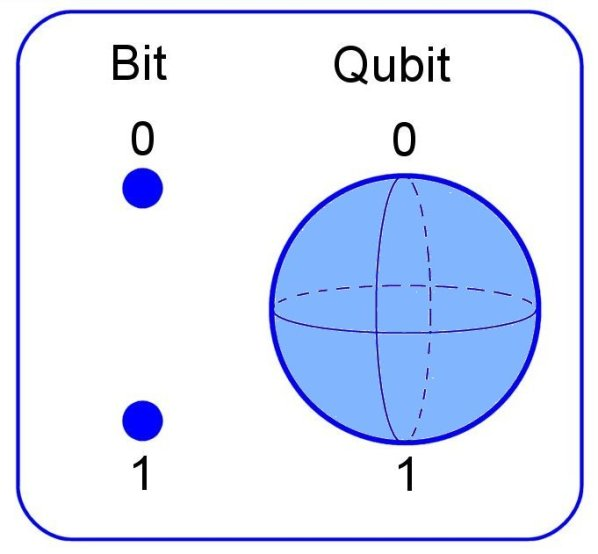
\includegraphics[
        width=\textwidth,
        keepaspectratio
    ]{bit.jpg}
\end{minipage}

\end{Center}




\section{1.3. Qubits fotónicos y su medición}

\begin{Center}


En una implementación fotónica de
\textbf{BB84}, la información cuántica
se codifica en la polarización
de los fotones, mediante:
 \vspace{-0.4cm}
 
\[
|0\rangle=|\leftrightarrow\rangle,
\qquad
|1\rangle=|\updownarrow\rangle
\]

que representan las polarizaciones
horizontal y vertical


Se mide mediante un
divisor de haz polarizante (PBS),
que dirige el fotón hacia uno de
dos detectores.

\medskip

La base de medición puede cambiarse
utilizando elementos ópticos,
como las placas de media onda.

\end{Center}



\section{1.4. Bases de medición cuántica}

\begin{Center}

\begin{minipage}[c]{0.53\textwidth}
\small

El resultado de medir un qubit
depende de la base de medición
que utilicemos.
\vspace{0.3cm}


\textbf{Base computacional ($Z$):}

\[
\mathcal{B}_Z=\{|0\rangle,|1\rangle\}
\]

\vspace{0.3cm}

\textbf{Base diagonal ($X$):}

\[
|+\rangle=\frac{|0\rangle+|1\rangle}{\sqrt{2}}
\]


\[
|-\rangle=\frac{|0\rangle-|1\rangle}{\sqrt{2}}
\]
\end{minipage}
\hfill
\begin{minipage}[c]{0.43\textwidth}
    \centering

    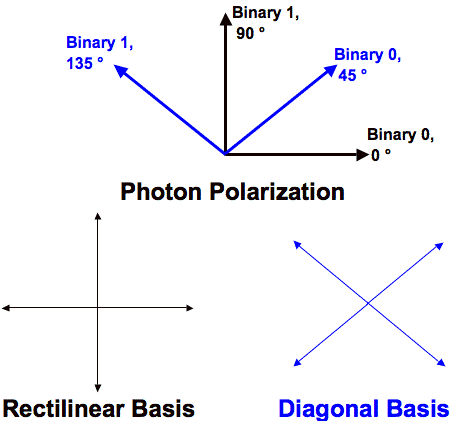
\includegraphics[
        width=\textwidth,
        keepaspectratio
    ]{images.png}

    \vspace{0.2cm}

    {\scriptsize
    Bases rectilínea y diagonal
    de polarización.
    }

\end{minipage}

\end{Center}


\section{1.5. Protocolo BB84}

\begin{Center}

\centering

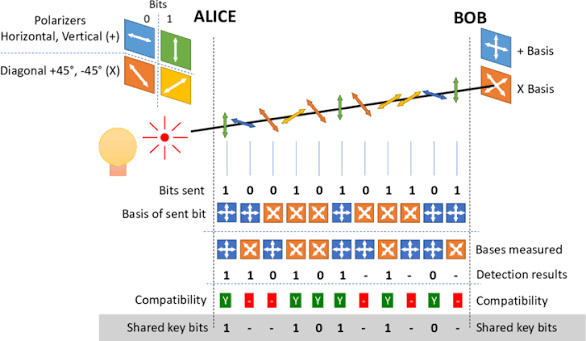
\includegraphics[
    width=\textwidth,
    height=\textheight,
    keepaspectratio
]{Alice_Bob.png}

\end{Center}


\section{1.6. Seguridad del protocolo BB84}

\begin{Center}

\begin{minipage}[c]{0.53\textwidth}
\small

Eve intercepta y mide
los fotones, alterarando sus
estados al elegir una base incorrecta.

\medskip

Alice y Bob pueden detectar estos errores
mediante el QBER:

\[
QBER=\frac{N_{\text{errores}}}
{N_{\text{bits comparados}}}
\]

Para una interceptación total
con mediciones aleatorias:

\[
\boxed{QBER=25\%}
\]

\end{minipage}
\hfill
\begin{minipage}[c]{0.43\textwidth}
    \centering
    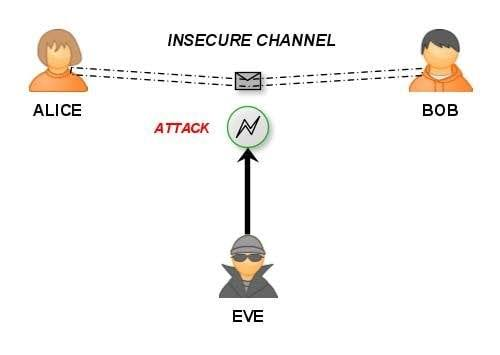
\includegraphics[
        width=\textwidth,
        keepaspectratio
    ]{eve.jpeg}
\end{minipage}

\end{Center}


\section{1.7. Entrelazamiento cuántico}

\begin{Center}

\begin{minipage}[c]{0.53\textwidth}
\small

Dos qubits están entrelazados
cuando su estado conjunto no puede
describirse como el producto de
estados individuales.

\medskip

Un ejemplo es el estado de Bell:

\[
\boxed{
|\Phi^+\rangle =
\frac{|00\rangle+|11\rangle}{\sqrt{2}}
}
\]

Al medir ambos qubits en la base
computacional, sus resultados
están perfectamente correlacionados.

\end{minipage}
\hfill
\begin{minipage}[c]{0.43\textwidth}
    \centering
    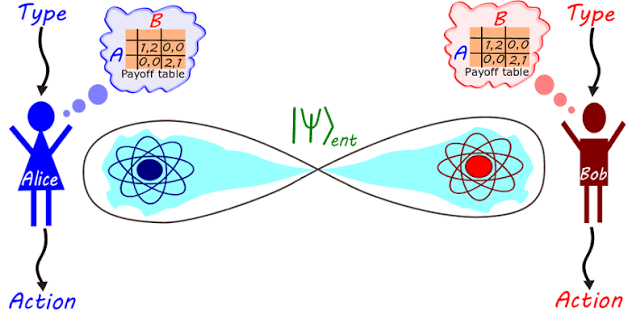
\includegraphics[
        width=\textwidth,
        keepaspectratio
    ]{entanglement.png}
\end{minipage}

\end{Center}


\section{1.8. Estados de Bell}

\begin{Center}

\centering

Los cuatro estados de Bell
forman una base ortonormal de estados
entrelazados para un sistema de dos qubits.\\

% PRIMERA COLUMNA
\begin{minipage}[c]{0.47\textwidth}
\centering

\[
\boxed{
|\Phi^{+}\rangle =
\frac{|00\rangle+|11\rangle}{\sqrt{2}}
}
\]

\[
\boxed{
|\Phi^{-}\rangle =
\frac{|00\rangle-|11\rangle}{\sqrt{2}}
}
\]

\end{minipage}
\hfill
% SEGUNDA COLUMNA
\begin{minipage}[c]{0.47\textwidth}
\centering

\[
\boxed{
|\Psi^{+}\rangle =
\frac{|01\rangle+|10\rangle}{\sqrt{2}}
}
\]

\[
\boxed{
|\Psi^{-}\rangle =
\frac{|01\rangle-|10\rangle}{\sqrt{2}}
}
\]

\end{minipage}

\vspace{0.7cm}

\small
En la teleportación cuántica,
Alice realiza una medición en la base de Bell
para determinar qué corrección debe aplicar Bob.

\end{Center}


\section{1.9. Estado inicial de la teleportación}

\begin{Center}

\small
Alice desea teleportar un estado desconocido
a Bob utilizando un par entrelazado.

\vspace{0.5cm}

% COLUMNA IZQUIERDA
\begin{minipage}[c]{0.46\textwidth}
\centering
\small

\textbf{Qubit desconocido (Alice):}

\[
|\psi\rangle_1 =
\alpha|0\rangle_1+\beta|1\rangle_1
\]

\vspace{0.5cm}

\textbf{Par entrelazado (Alice y Bob):}

\[
|\Phi^+\rangle_{23} =
\frac{|00\rangle_{23}+|11\rangle_{23}}
{\sqrt{2}}
\]

\end{minipage}
\hfill
% COLUMNA DERECHA
\begin{minipage}[c]{0.51\textwidth}
\centering
\small

\textbf{Estado conjunto:}

\[
|\Psi_0\rangle =
|\psi\rangle_1\otimes|\Phi^+\rangle_{23}
\]

\vspace{0.3cm}

\[
\boxed{
\begin{aligned}
|\Psi_0\rangle = \frac{1}{\sqrt{2}}\big(
&\alpha|000\rangle+\alpha|011\rangle\\
&+\beta|100\rangle+\beta|111\rangle
\big)
\end{aligned}
}
\]

\end{minipage}

\end{Center}


\section{1.10. Cambio a la base de Bell}

\begin{Center}

% COLUMNA IZQUIERDA
\begin{minipage}[c]{0.43\textwidth}
\centering
\small

\textbf{Estado inicial:}

\[
\begin{aligned}
|\Psi_0\rangle =
\frac{1}{\sqrt{2}}\big(
&\alpha|000\rangle+\alpha|011\rangle\\
&+\beta|100\rangle+\beta|111\rangle
\big)
\end{aligned}
\]

\end{minipage}
\hfill
% COLUMNA DERECHA
\begin{minipage}[c]{0.54\textwidth}
\centering
\small

\textbf{Expansión en la base de Bell:}

\[
\begin{aligned}
|\Psi_0\rangle=\frac{1}{2}\Big[
&|\Phi^+\rangle_{12}
(\alpha|0\rangle+\beta|1\rangle)_3\\[4pt]
+&|\Phi^-\rangle_{12}
(\alpha|0\rangle-\beta|1\rangle)_3\\[4pt]
+&|\Psi^+\rangle_{12}
(\beta|0\rangle+\alpha|1\rangle)_3\\[4pt]
+&|\Psi^-\rangle_{12}
(\alpha|1\rangle-\beta|0\rangle)_3
\Big]
\end{aligned}
\]

\end{minipage}

\end{Center}



\section{1.11. Correcciones de la teleportación}

\begin{Center}

\small
Alice realiza una medición en la base de Bell
sobre sus dos qubits y comunica el resultado
a Bob mediante dos bits clásicos.

\vspace{0.5cm}

\begin{center}
\scriptsize
\setlength{\tabcolsep}{5pt}
\renewcommand{\arraystretch}{1.3}

\begin{tabular}{c c c c}
\hline
\textbf{Bell} &
\textbf{Bits $(c_1c_0)$} &
\textbf{Estado de Bob} &
\textbf{Corrección} \\
\hline

$|\Phi^+\rangle$ & $00$ &
$|\psi\rangle$ & $I$ \\

$|\Phi^-\rangle$ & $01$ &
$Z|\psi\rangle$ & $Z$ \\

$|\Psi^+\rangle$ & $10$ &
$X|\psi\rangle$ & $X$ \\

$|\Psi^-\rangle$ & $11$ &
$XZ|\psi\rangle$ & $ZX$ \\

\hline
\end{tabular}
\end{center}

\vspace{0.5cm}

Bob aplica $Z$ si $c_0=1$
y $X$ si $c_1=1$.

\vspace{0.4cm}

Después de aplicar las correcciones,
Bob recupera el estado original:

\[
\boxed{
|\psi\rangle_B =
\alpha|0\rangle+\beta|1\rangle
}
\]

\end{Center}




\section{1.12. Teorema de no clonación}

\begin{Center}

% COLUMNA IZQUIERDA
\begin{minipage}[c]{0.47\textwidth}
\centering
\small
Supongamos una operación unitaria $U$
que puede clonar los estados base:

\[
\begin{aligned}
U(|0\rangle|b\rangle)&=|00\rangle\\
U(|1\rangle|b\rangle)&=|11\rangle
\end{aligned}
\]

\vspace{0.2cm}

Por linealidad sabemos que,
\vspace{-0.2cm}

\[
\begin{aligned}
U(|+\rangle|b\rangle)
&=\frac{1}{\sqrt{2}}
U\big((|0\rangle+|1\rangle)|b\rangle\big)\\
&=\frac{|00\rangle+|11\rangle}{\sqrt{2}}
\end{aligned}
\]

\end{minipage}
\hfill
% COLUMNA DERECHA
\begin{minipage}[c]{0.49\textwidth}
\centering
\small
Para $|+\rangle=(|0\rangle+|1\rangle)/\sqrt{2}$,
deberíamos obtener:

\[
\begin{aligned}
|+\rangle|+\rangle
=\frac{1}{2}\big(
&|00\rangle+|01\rangle\\
&+|10\rangle+|11\rangle
\big)
\end{aligned}
\]


\[
\boxed{
U(|+\rangle|b\rangle)
\neq |+\rangle|+\rangle
}
\]

\medskip

\textbf{No existe un clonador
cuántico universal.}

\end{minipage}

\end{Center}


\section{1.13. Teleportación y no clonación}

\begin{Center}

% COLUMNA IZQUIERDA
\begin{minipage}[c]{0.47\textwidth}
\centering
\small

\textbf{Teorema de no clonación}

\medskip

No es posible crear una copia
perfecta de un estado cuántico
arbitrario y desconocido.

\[
|\psi\rangle|b\rangle
\not\longrightarrow
|\psi\rangle|\psi\rangle
\]

\medskip

La clonación conservaría el estado
original y produciría una
segunda copia idéntica.

\end{minipage}
\hfill
% COLUMNA DERECHA
\begin{minipage}[c]{0.47\textwidth}
\centering
\small

\textbf{Teleportación cuántica}

\medskip

La medición de Bell de Alice
destruye el estado original
como qubit independiente.

\medskip

Bob aplica la corrección indicada
por los dos bits clásicos:

\[
\boxed{
U_k|\psi_k\rangle_3=|\psi\rangle_3
}
\]

\medskip

El estado se \textbf{transfiere},
pero nunca existen dos copias
independientes.

\end{minipage}

\end{Center}


\section{1.14. Fidelidad de la teleportación}

\begin{Center}

% COLUMNA IZQUIERDA
\begin{minipage}[c]{0.47\textwidth}
\centering
\small

Mide qué tan cercano es el
estado recibido por Bob al
estado original de Alice.
\vspace{-0.2cm}


\[
\boxed{
F=\langle\psi|\rho_B|\psi\rangle
}
\]

\vspace{0.2cm}

Donde $\rho_B$ es la matriz de
densidad del estado recibido.

\end{minipage}
\hfill
% COLUMNA DERECHA
\begin{minipage}[c]{0.47\textwidth}
\centering
\small

\[
F=1
\quad\text{Teleportación perfecta}
\]

\vspace{-0.5cm}

\[
F<1
\quad\text{Teleportación imperfecta}
\]

Para estados puros desconocidos
distribuidos uniformemente,
el límite clásico promedio es:

\[
\boxed{\overline{F}_{\mathrm{clásica}}
\leq\frac{2}{3}}
\]

\end{minipage}

\end{Center}

\chapter{2. Simulación y resultados}

\section{2.1. Implementación en Google Colab}

\begin{Center}

\begin{minipage}[t]{0.47\textwidth}
\small

\textbf{Simulación de BB84}

\medskip

Utilizamos Python y NumPy para reproducir
las elecciones de bases y los resultados
de las mediciones.

\begin{itemize}
    \item Canal ideal sin espía.
    \item Interceptación y reenvío de Eva.
    \item Probabilidad de interceptación variable.
    \item Cálculo del QBER y de las tasas de clave.
\end{itemize}

\end{minipage}
\hfill
\begin{minipage}[t]{0.47\textwidth}
\small

\textbf{Circuito de teleportación}

\medskip

Construimos el circuito con Qiskit
y comprobamos su funcionamiento
en dos condiciones:

\begin{itemize}
    \item Simulación ideal con Aer.
    \item Ejecución real en IBM Kingston.
\end{itemize}

\medskip

Guardamos las gráficas y los resultados
en archivos PNG, CSV y JSON.

\end{minipage}

\end{Center}


\section{2.2. Simulación de la interceptación parcial}

\begin{Center}

\begin{minipage}[c]{0.55\textwidth}
\small

\begin{enumerate}
    \item Alice genera bits y bases al azar.
    \item Eva intercepta cada señal
    con probabilidad $f$.
    \item Si interviene, mide en una base
    aleatoria y reenvía el estado obtenido.
    \item Bob mide en su propia base.
    \item Alice y Bob conservan las posiciones
    donde sus bases coinciden.
\end{enumerate}

\end{minipage}
\hfill
\begin{minipage}[c]{0.41\textwidth}
\small
\centering

\textbf{Configuración del barrido}

\medskip

$10\,000$ señales por prueba.

\medskip

$f=0,\;0.1,\;0.2,\ldots,1$.

\medskip

Semillas: 2026 a 2036.

\medskip

Canal sin ruido adicional.

\[
Q=\frac{N_{\text{errores}}}
{N_{\text{bits cribados}}}
\]

\end{minipage}

\medskip



\end{Center}

\section{2.3. QBER frente a la interceptación}

\begin{Center}

\textbf{Predicción para un canal sin ruido adicional}
\quad \(Q = f/4\)

\medskip

\noindent
\begin{minipage}[c]{0.62\textwidth}
    \centering
    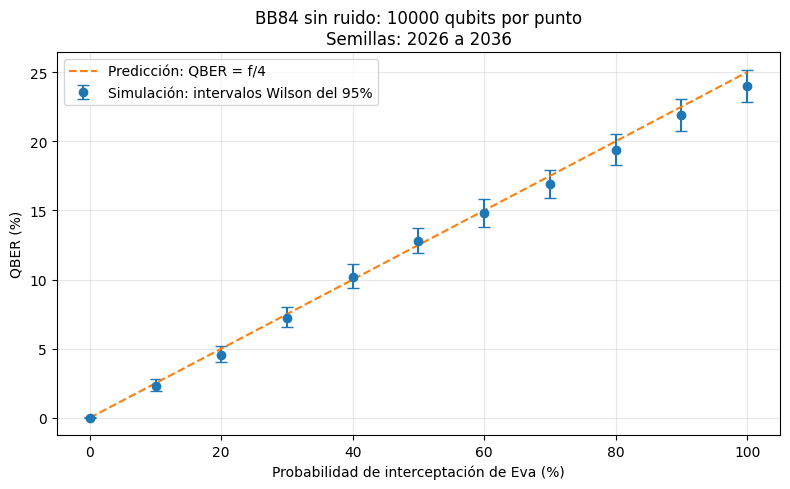
\includegraphics[
        width=\linewidth,
        height=1.5\textheight,
        keepaspectratio
    ]{Resultados/BB84_QBER_con_incertidumbre.png}
\end{minipage}\hfill
\begin{minipage}[c]{0.35\textwidth}
    \centering
    \small
    \textbf{Resultados del barrido}\par
    \medskip

    \setlength{\tabcolsep}{4pt}
    \renewcommand{\arraystretch}{1.2}
    \begin{tabular}{@{}cc@{}}
        \textbf{Eva intercepta} & \textbf{QBER} \\
        \hline
        0\%   &  0.00\% \\
        50\%  & 12.78\% \\
        100\% & 23.98\% \\
    \end{tabular}
\end{minipage}

\smallskip


\end{Center}


\section{2.4. Tasas de clave}

\begin{Center}
\centering
\small

\textbf{Tasa secreta estimada}\quad
\( R_{\mathrm{secreta}} =
   \frac{N_{\mathrm{cribados}}}{N_{\mathrm{enviados}}}
   \max\{0,\,1-2h_2(Q)\} \)

\smallskip

\noindent
\begin{minipage}[c]{0.60\textwidth}
    \centering
    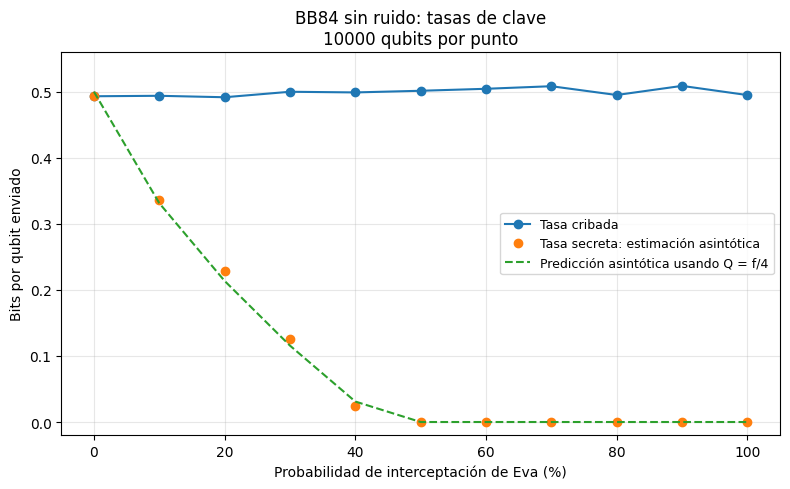
\includegraphics[
        width=\linewidth,
        height=1.8\textheight,
        keepaspectratio
    ]{Resultados/BB84_tasas_de_clave.png}
\end{minipage}\hfill
\begin{minipage}[c]{0.37\textwidth}
    \centering
    \textbf{Bits por señal enviada}\par
    \smallskip

    \setlength{\tabcolsep}{3pt}
    \renewcommand{\arraystretch}{1.15}
    \begin{tabular}{@{}rcc@{}}
        \textbf{Eva} & \textbf{Cribada} & \textbf{Secreta est.} \\
        \hline
         0\,\% & 0.4932 & 0.4932 \\
        40\,\% & 0.4990 & 0.0240 \\
        50\,\% & 0.5015 & 0.0000 \\
    \end{tabular}
\end{minipage}

\smallskip


\end{Center}


\section{2.5. Circuito de teleportación en Qiskit}

\begin{Center}

\centering

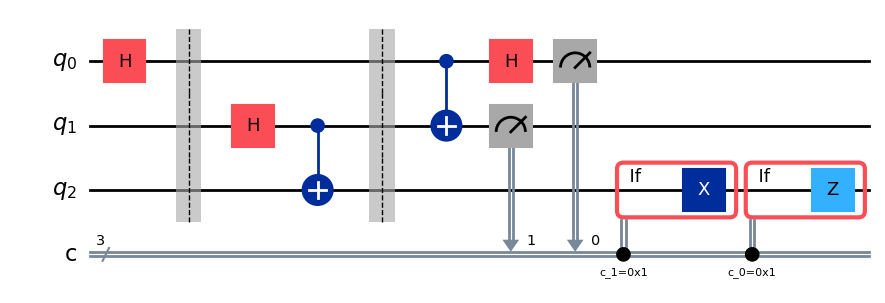
\includegraphics[
    width=0.88\textwidth,
    height=0.56\textheight,
    keepaspectratio
]{Resultados/teleportacion_circuito_logico.png}
\par
{\centering\footnotesize
Circuito de teleportación para el estado de entrada \( |+\rangle \).
\par}
\medskip

\begin{minipage}[t]{0.47\textwidth}
\small

\textbf{Distribución de los qubits}

\begin{itemize}
    \item $q_0$: estado de entrada de Alice.
    \item $q_1$: mitad del par de Bell de Alice.
    \item $q_2$: mitad del par de Bell de Bob.
\end{itemize}

\end{minipage}
\hfill
\begin{minipage}[t]{0.47\textwidth}
\small

\textbf{Correcciones de Bob}

\begin{itemize}
    \item Si $c_1=1$, aplica $X$.
    \item Si $c_0=1$, aplica $Z$.
\end{itemize}



\end{minipage}

\medskip



\end{Center}


\section{2.6. Verificación con seis estados}

\begin{Center}
\vspace{-.5cm}
\[
|0\rangle,\quad |1\rangle,\quad
|+\rangle,\quad |-\rangle,\quad
|+i\rangle,\quad |-i\rangle
\]

\medskip

\begin{minipage}[c]{0.52\textwidth}
\small

Preparamos cada estado mediante una operación $U$.

\medskip

Después de la teleportación, aplicamos
$U^\dagger$ sobre el qubit de Bob
y lo medimos.

\[
U^\dagger|\psi\rangle=|0\rangle
\]

Una verificación correcta produce $0$,
incluso cuando teleportamos $|1\rangle$.

\end{minipage}
\hfill
\begin{minipage}[c]{0.44\textwidth}
\small
\centering

\textbf{Simulación ideal}

\medskip

1024 ejecuciones por estado.

\[
\widehat{F}
=
\frac{N_{\text{verificaciones correctas}}}
{N_{\text{ejecuciones}}}
\]

\[
\boxed{\widehat{F}=1.0000}
\]

Para los seis estados.

\end{minipage}

\medskip


\end{Center}


\section{2.7. Conexión y ejecución en IBM Quantum}

\begin{Center}

\begin{minipage}[c]{0.58\textwidth}
\small

\begin{enumerate}
    \item Conectamos Google Colab con
    Qiskit Runtime mediante la API key
    y el CRN de la instancia.

    \item Seleccionamos un procesador
    con mediciones intermedias y
    operaciones condicionadas.

    \item Adaptamos los circuitos a sus
    compuertas y conexiones mediante
    la transpilación.

    \item Enviamos los seis circuitos
    en un mismo trabajo y recuperamos
    los conteos.
\end{enumerate}

\end{minipage}
\hfill
\begin{minipage}[c]{0.38\textwidth}
\small
\centering

\textbf{Procesador utilizado}

\medskip

\texttt{ibm\_kingston}

\medskip

6 circuitos.

\medskip

1024 ejecuciones por estado.

\medskip

\textbf{Transpilación}

Nivel de optimización: 1.

Semilla: 2026.

\end{minipage}

\medskip

{\scriptsize
Job ID: \texttt{dboelu44148s739stt70}.

}

\end{Center}


\section{2.8. Circuito adaptado a IBM Kingston}

\begin{Center}

\begin{minipage}[c]{0.50\textwidth}
\centering

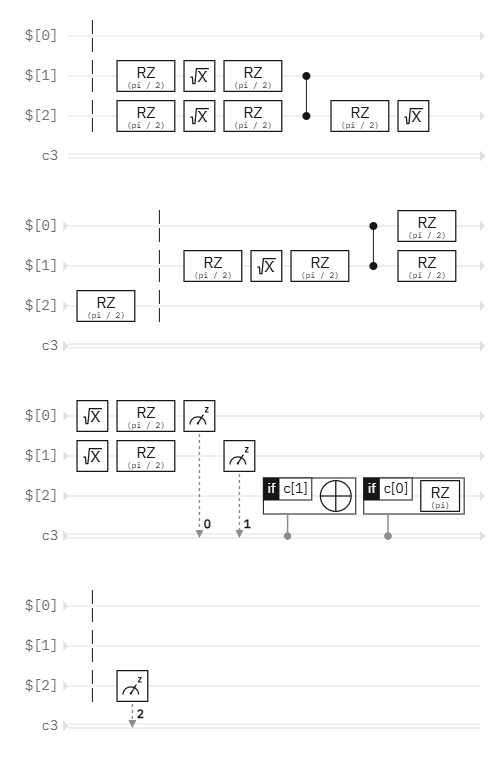
\includegraphics[
    width=\linewidth,
    height=1\textheight,
    keepaspectratio
]{Resultados/teleportacion_circuito_IBM_vertical.png}

\end{minipage}
\hfill
\begin{minipage}[c]{0.46\textwidth}
\small

La transpilación expresa las operaciones
mediante las compuertas disponibles
en el procesador.

\medskip

\begin{itemize}
    \item El circuito continúa de izquierda
    a derecha y de arriba hacia abajo.

    \item Las mediciones de Alice
    controlan las correcciones de Bob.

    \item La última medición registra
    la verificación en $c_2$.
\end{itemize}

\medskip

Los tres qubits pertenecen
al mismo procesador.

\end{minipage}

\medskip

{\scriptsize
Imagen del trabajo propio en IBM Quantum Platform.
}

\end{Center}


\section{2.9. Resultados en IBM Kingston}

\begin{Center}

\begin{minipage}[c]{0.64\textwidth}
\centering

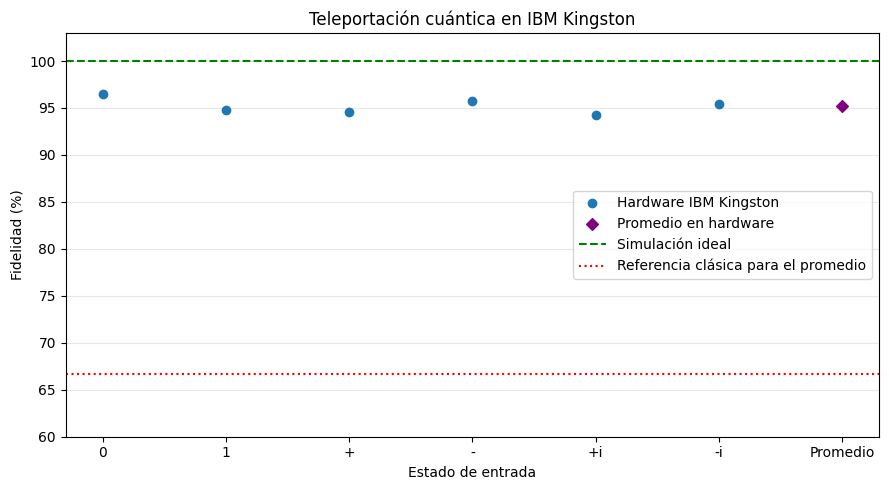
\includegraphics[
    width=\linewidth,
    height=1.7\textheight,
    keepaspectratio
]{Resultados/teleportacion_comparacion_hardware.png}

\end{minipage}
\hfill
\begin{minipage}[c]{0.32\textwidth}
\small
\centering

\textbf{Fidelidad promedio}

\[
\boxed{\overline{F}=95.20\%}
\]

5849 verificaciones correctas
de 6144 ejecuciones.

\medskip

Valores por estado:
de $94.24\%$ a $96.48\%$.

\medskip

Simulación ideal: $100\%$.

\end{minipage}

\medskip

{\small
La medición incluye las imperfecciones
de preparación, del circuito y de lectura.
}

\medskip

{\scriptsize
La referencia clásica de $2/3$ corresponde al promedio
bajo el criterio de estimación de estados desconocidos.
}

\end{Center}


\section{2.10. Conclusiones de la implementación}

\begin{Center}

\begin{minipage}[t]{0.47\textwidth}
\small

\textbf{BB84}

\medskip

La interceptación introduce errores
en las claves cribadas.

\[
Q \approx \frac{f}{4}
\]

La tasa cribada permanece cerca de $0.5$,
pero la tasa secreta estimada disminuye
al aumentar el QBER.

\medskip

El modelo considera interceptación y reenvío
sin ruido adicional.

\end{minipage}
\hfill
\begin{minipage}[t]{0.47\textwidth}
\small

\textbf{Teleportación}

\medskip

El simulador ideal recuperó correctamente
los seis estados de prueba.

\medskip

En IBM Kingston obtuvimos una fidelidad
promedio de $95.20\%$.

\medskip

El resultado corresponde a un trabajo
en un solo procesador.
Repetirlo permitiría estudiar
su variación entre ejecuciones.

\end{minipage}

\end{Center}


\chapter{Gracias!}

\end{document}
